\begin{Exemple}[Organiser vscode]

    Une fois configuré, votre environnement de travail devrait ressembler à ceci : 

    \begin{center}
        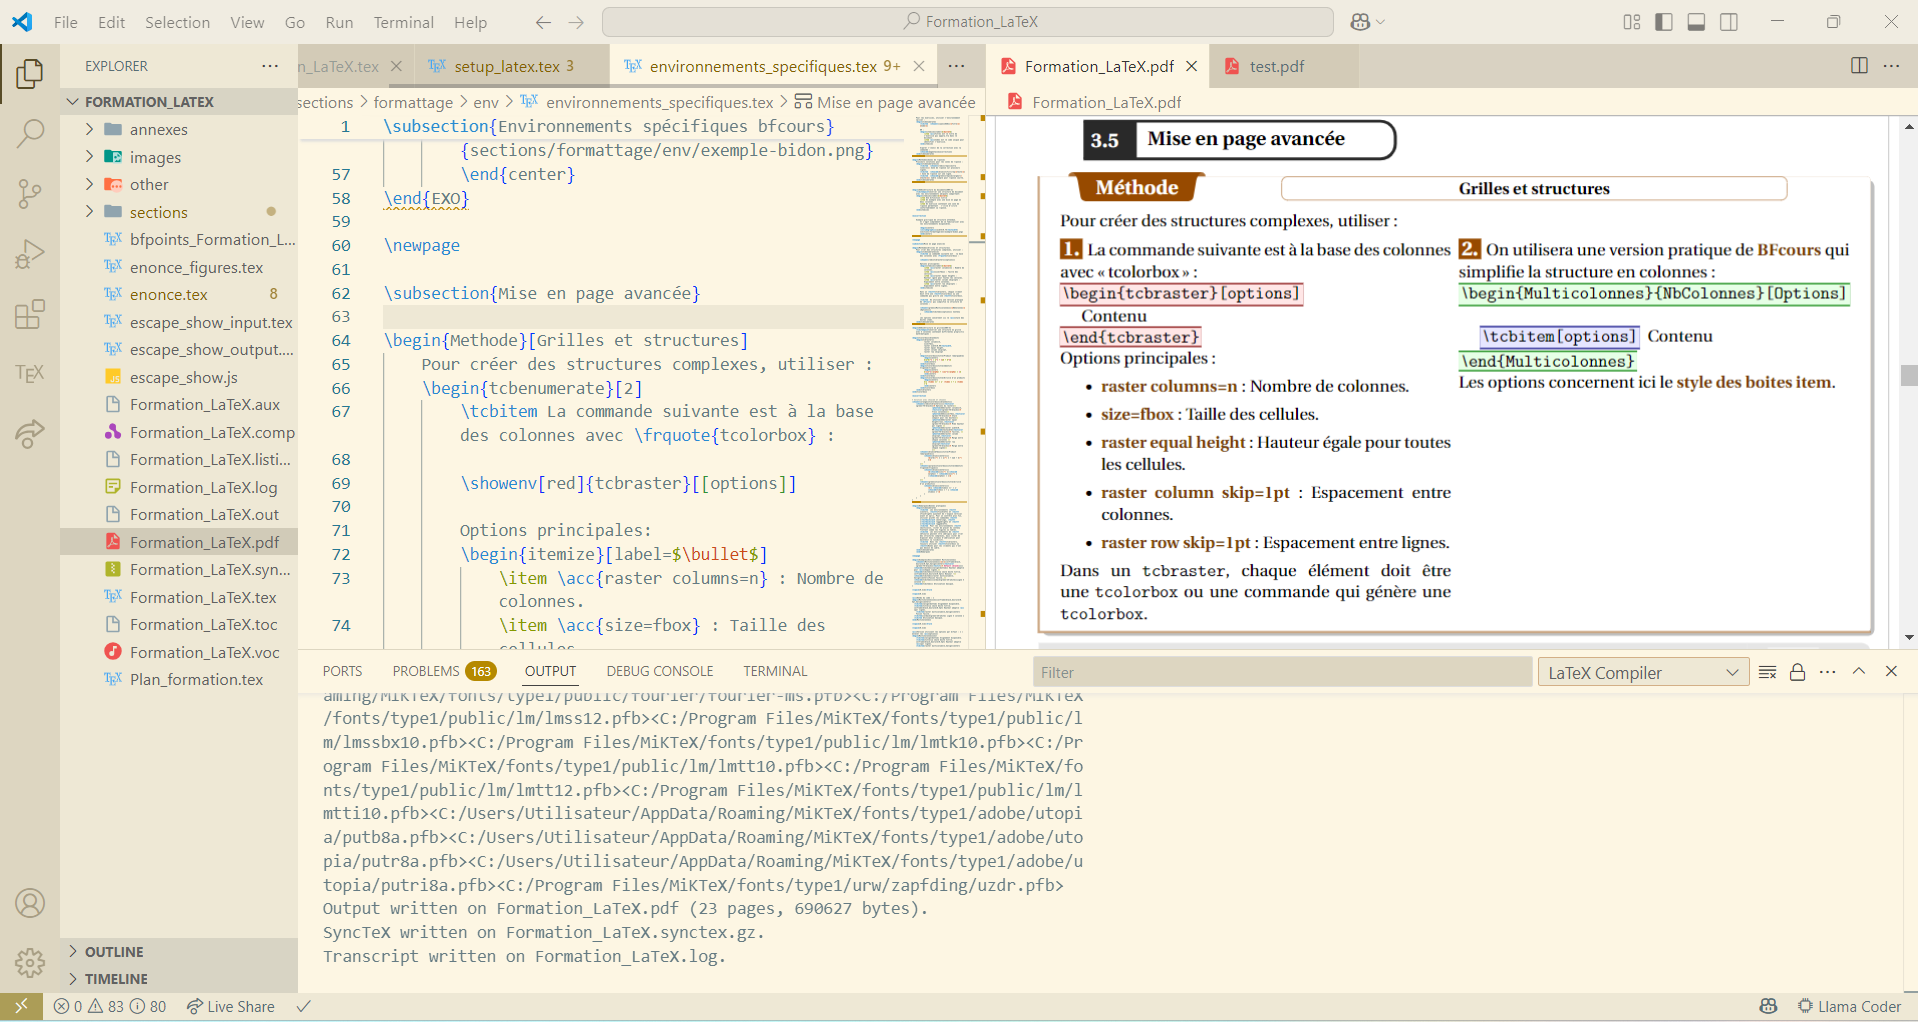
\includegraphics[width=0.8\textwidth]{images/IDE/VSCode_use.png}
    \end{center}

    On observe : 
    \begin{tcbenumerate}[2]
        \tcbitem Options générales
        \tcbitem Barre de recherche
        \tcbitem Géométrie voulue pour le terminal
        \tcbitem La \acc{sidebar}
        \tcbitem La zone d'exploration ( fichiers, extensions, recherche sur fichiers multiples )
        \tcbitem Onglets
        \tcbitem Zone de saisie principale
        \tcbitem Zone d'affichage ou de saisie secondaire
        \tcbitem Terminal - permet également d'afficher les logs : 

        \bouton{OUTPUT}$\rightarrow$\bouton{Latex Compiler}
    \end{tcbenumerate}
\end{Exemple}